\chapter{Preliminaries}\label{sec:preliminaries}

In this chapter, we will give a short introduction into graph theory, shortest path algorithms, random graph models as well as Markov chains.
We denote the set of positive real numbers by $\sRpos$, the set of consecutive whole numbers $\setc{i}{a \leq i \leq n, \i in \sZ}$ by $[a..b]$ and write $[n]$ as shorthand for $[1..n]$.
$\unif(X)$ refers to a uniform distribution over the ground set $X$.

\iffalse
\begin{table}[h]
  \centering
  \begin{tabular}{lll}
    \toprule
      Notation & Description & Defined in \\
    \midrule
      $\sRpos$ & Set of positive real numbers & \\
      $[n]$ & $\setc{i}{1 \leq i \leq n, i \in \sN}$ \\
      $[a..b]$ & $\setc{i}{a \leq i \leq b, i \in \sZ} \subseteq \sZ$ \\
      $\unif(X)$ & Uniform distribution over set $X$ & \\ 
      $d(u, v)$ & Length of a shortest \path{u}{v} & \cref{def:shortest_path} \\
      $\spt(u)$ & Shortest path tree rooted in $u$ & \cref{def:shortest_path_tree} \\
      $\pot$ & Potential function $\pot\colon V \rightarrow \sR$ & \cref{def:potentials} \\
      $\wpot$ & Potential weight function & \cref{def:potentials} \\
      $\diam$ & Diameter of $G$ or a shortest path tree & \cref{def:diameter} \\
      $\algdk$ & \algdk's SSSP algorithm & \cref{algo:dijkstra} \\
      $\algbf$ & \algbf's SSSP algorithm & \cref{algo:bellmanford} \\
      $\algjs$ & \algjs's APSP algorithm & \cref{algo:johnson} \\
      $\rtime_A$ & Running time of algorithm $A$ & \\
      $\gnp(n, \degavg)$ & Graph from the Gilbert model & \cref{sec:gnp} \\
      $\dsf(n, \degavg)$ & Graph from the DirectedScaleFree model & \cref{sec:dsf} \\
      $\rhg(n, \degavg)$ & Graph from the Hyperbolic graph model & \cref{sec:rhg} \\
      \mixtime & Mixing time of a \markov & \cref{def:mixing_time} \\
    \bottomrule
  \end{tabular}
  \caption{
    Notations used in this thesis.
  }
  \label{tab:notations}
\end{table}
\fi

\section{Graph Theory}
We only focus on weighted directed graphs as negative weights in undirected graphs are significantly harder to handle~\cite{TJoin}. 

\begin{definition}[Directed Graph]
  A directed graph $G$ is a tuple $(V,E)$ where $V$ is a finite set of nodes (or vertices) and $E \subseteq V \times V$ is a set of directed edges.
  For edge $(u, v) \in E$, we call $u$ the source and $v$ the target of the edge.
  If unambiguous from context, we use $n \Def |V|$ and $m \Def |E|$ to denote the number of nodes and edges. 
\end{definition}

\begin{definition}[Weight Function]
  For graph $G = (V, E)$, a weight function $w\colon E \rightarrow \wInt$ assigns each edge a weight from $\wInt$ (typically $\wInt \subseteq \sZ$ or $\wInt \subseteq \sR$).
  For edge $e = (u, v) \in E$, we call $w(e) = w(u, v)$ its edge weight.
\end{definition}

\noindent Unless further specified, for the rest of the thesis, $G = (V, E)$ refers to a graph with nodes $V$ and edges $E$ and $w\colon E \rightarrow \wInt$ to a weight function defined on $G$ with $\wInt \subseteq \sR$.


\begin{definition}[Path]
  We call $P = (v_1, \ldots, v_k) \in V^k$ a $k$-path (or just path), if all edges $(v_i, v_{i + 1}),\,i \in [k - 1]$ exist in $E$.
  We call $P$ a \path{u}{v} if $v_1 = u$ and $v_k = v$ and say $u$ can reach $v$.
\end{definition} 

\begin{definition}[Cycle]
  A $(k + 1)$-path $(v_1, \ldots, v_{k + 1})$ is a $k$-cycle if $v_1 = v_{k + 1}$.  
\end{definition}

\noindent We call a path or cycle \emph{simple} if no node appears more than once (for a cycle this excludes $v_1 = v_{k + 1}$).
We denote the number of edges in a path (or cycle) $P$ by $|P|$.
An acyclic graph is a graph with no cycles.

\begin{definition}[Tree]
  $G$ is a (rooted) tree if it is acyclic and there exists $u \in V$ that can reach every other node $v \in V \setminus \set{u}$. 
\end{definition}


\begin{definition}[SCC]
  We call a subset of nodes $S \subseteq V$ a strongly connected component (SCC) if for every $u, v \in S$, $u$ can reach $v$ and vice-versa.
  We say $G$ is strongly connected if $V$ is a SCC.
\end{definition}

\begin{definition}[Subgraph]
  We call $G' = (S, E')$ a subgraph of $G$, if $S \subseteq V$ and $E' \subseteq E \cap S^2$.
  If $E' = E \cap S^2$, we call $G'$ the subgraph induced by $S$.
  If $G'$ is a tree, we call $G'$ a subtree of $G$.
\end{definition}

\begin{definition}[Weight of a Path]
  For a $k$-path $P = (v_1, \ldots, v_k)$, we overload $w$ and write \[
    w(P) = \sum_{i = 1}^{k - 1}w(v_i, v_{i + 1})
  \] to denote its weight. 
\end{definition}

\noindent We also allow $1$-paths, \ie $P = (u)$ and set its weight to $w(P) = 0$.

\begin{definition}[Shortest Path]\label{def:shortest_path}
  A shortest \path{u}{v} is defined as a \path{u}{v} with minimum weight among all possible \paths{u}{v}.
  For an ordered pair of vertices $(u, v) \in V^2$, we denote the distance from $u$ to $v$ by \[
    d_{G, w}(u, v) = d(u, v) = \begin{cases}
      \min\setc{w(P)}{\text{$P$ is a \path{u}{v}}} & \text{if $u$ can reach $v$} \\
      \infty & \text{otherwise}
    \end{cases}
  \] 
\end{definition}

\noindent In the unweighted case, \ie $w\colon E \rightarrow \set{1}$, the weight of a shortest \path{u}{v} $P$ is equivalent to the number of edges $|P|$ in it and we only need to traverse the graph using \textsc{BreadthFirstSearch} (\bfs)~\cite{zuse1972plankalkuel} to compute a shortest path. 
For general weights, however, the length of a shortest \path{u}{v} can be arbitrary, even negative if we allow negative weights which can lead to complications.

\begin{figure}[t]
  \centering
  \begin{tikzpicture}
    \node[vertex] (u) at (0,0) {$u$};
    \node[vertex] (x) at (2,0) {$x$};
    \node[vertex] (y) at (4,0) {$y$};
    \node[vertex] (v) at (6,0) {$v$};

    \edge{u}{x}{$1$}{}{};
    \edge{x}{y}{$-1$}{}{bend left, broken};
    \edge{y}{x}{$0$}{}{bend left, broken};
    \edge{y}{v}{$1$}{}{};
    \edge{u}{v}{$3$}{}{bend left};
\end{tikzpicture}

  
  \caption{
    A graph with $4$ nodes containing a negative cycle $(x, y, x)$. 
  }
  \label{fig:neg_cycle}
\end{figure}

\begin{definition}[Negative Cycle] 
  A cycle $C$ is a negative cycle if $w(C) < 0$.
\end{definition}

\noindent The notion of a shortest path only makes sense if there is no negative cycle present.
For that, consider \cref{fig:neg_cycle}. 
There exist two simple \paths{u}{v}: $P_1 = (u, v)$ and $P_2 = (u, x, y, v)$ with $w(P_1) = 3 > 1 = w(P_2)$.
Thus, $P_2$ is a shortest \textbf{simple} \path{u}{v}.
The cycle $C = (x, y, x)$ however has weight $w(C) = -1$ and is thus negative.
We can now traverse $C$ multiple times instead of once (as in $P_2$) to continuously decrease the weight of $P_2$.
Therefore, the weight of a shortest \path{u}{v} is unbounded and there is no finite shortest \path{u}{v}.

\begin{definition}[Consistent Weight Function]
  We say $(G, w)$ are consistent if no negative cycles exist.
\end{definition}

\noindent Hence, if we want to have reasonable shortest paths in a graph, we desire $(G,w)$ to be consistent.
The rest of the thesis focuses on checking for and maintaining consistency of $(G,w)$ under dynamic weight functions.


\section{Shortest Path Algorithms}
An important property of shortest paths is that they consists of shortest subpaths.

\begin{observation}\label{obs:shortest_paths_are_recursive}
  Let $P = (v_1, \ldots, v_k)$ be a shortest \path{v_1}{v_k}.
  Then $P_i = (v_1, \ldots, v_i)$ is a shortest \path{v_1}{v_i} for $i \in [k]$.
\end{observation}

\begin{definition}[Shortest Path Tree]\label{def:shortest_path_tree}
  For source node $u$, a shortest path tree $T$ from $u$, denoted by $\spt(u)$ is a subtree of $G$ such that \[
    d_{G, w}(u, v) = d_{T, w}(u, v) \quad\forall v \in V.
  \]  
\end{definition}

\noindent Note that if $G$ is strongly connected and has no negative cycles, due to \cref{obs:shortest_paths_are_recursive}, $\spt(u)$ exists for every $u \in V$ and contains every node in $V$.
Thus, $\spt(u)$ is well-defined if there is at most one shortest \path{u}{v} for every $v \in V$.
Note that in practice we often represent $\spt(u)$ implicitly as a distance mapping $D[v] = d(u, v)$ and do not explicitly store the structure of $\spt(u)$. 

\begin{definition}[SSSP Problem]
  The \sssp problem (SSSP) asks to compute $\spt(u)$ for a given source node $u$.
\end{definition}


\subsection{Dijkstra}

\begin{algorithm}[!tb]
  \caption{
    \algdk's SSSP algorithm~\cite{DBLP:journals/nm/Dijkstra59}.
  }
  \label{algo:dijkstra}

  \KwInput{graph $G = (V, E)$, weights $w\colon E \rightarrow \wInt,\,\,\wInt \subseteq \sRpos$, source node $u$}
  \KwOutput{$\spt(u)$}

  \BlankLine
  \For{$v \in V$}{
    $D[v] \gets \infty$\;
  }
  $D[u] \gets 0$\;
  \BlankLine
  $Q \gets \text{Min-}\textsc{PriorityQueue}$\;
  add $u$ to $Q$\;
  \While{$Q$ is not empty}{
    $v \gets$ node in $Q$ with minimum $D[v]$\;
    \For{$(v, x) \in E$}{
      \If{$D[v] + w(v, x) < D[x]$}{
        $D[x] \gets D[v] + w(v, x)$\;
        \lIf{$x \notin Q$}{
          add $x$ to $Q$
        }
      }
    }
  }
  \KwRet{$D$}\;
\end{algorithm}


One of the most famous algorithm for the weighted SSSP problem is \algdk's algorithm~\cite{DBLP:journals/nm/Dijkstra59}.
Described in~\cref{algo:dijkstra}, it starts from a given source node $u$ and stores the tentative distance $D[v]$ for every node $v \in V$.
In each round, we visit a node $v$ with smallest tentative distance. 
Then, we relax all its edges $(v, x)$ by checking whether the \path{u}{x} that visits $v$ directly before $x$ is shorter than the currently found \path{u}{x}.
To decide which node to visit, we keep all seen nodes that we have not visited yet in a Min-\textsc{PriorityQueue} which supports queries in logarithmic time.

The algorithm however relies on the fact that $w$ only assigns non-negative weights to all edges. 
If not, \algdk would still correctly output $\spt(u)$ if it exists but would not terminate if $G$ contains a negative cycle.
Thus, to use \algdk, we require all edges that we can traverse to have a non-negative weight.\footnote{
  If there exist negative edges but no negative cycle, \algdk would still correctly output $\spt(u)$ but not in the guaranteed runtime (see \cref{lem:dijkstra_runtime}).
}

\begin{lemma}\label{lem:dijkstra_runtime}
  For graph $G = (V, E)$ and weights $w\colon E \rightarrow \sRpos$, \algdk outputs a correct shortest path tree in time \[
    \rtime_{\algdk} = \Oh{m + n\log n}.\footnote{
      With standard priority queues, the runtime is rather $\Oh{(m + n)\log n}$. 
      Using a Fibonacci-Heap~\cite{FibonacciHeaps}, we get the stated runtime.
      Furthermore, if a Radix-Heap~\cite{RadixHeaps} is available, we can achieve a runtime of $\Oh{m + n}$.
    }
  \]
\end{lemma}


\subsection{BellmanFord}

\begin{algorithm}[t]
  \caption{
    \algbf's SSSP algorithm~\cite{Bel58, Ford56}.
  }
  \label{algo:bellmanford}

  \KwInput{graph $G = (V, E)$, weights $w\colon E \rightarrow \wInt$, source node $u$}
  \KwOutput{$\spt(u)$ or \negcycle}

  \BlankLine
  \For{$v \in V$}{
    $D[v] \gets \infty$\;
  }
  $D[u] \gets 0$\;
  \BlankLine
  \RepTimes{$|V| - 1$}{
    \For{$(u, v) \in E$}{
      \If{$D[u] + w(u, v) < D[v]$}{
        $D[v] = D[u] + w(u, v)$\;
      }
    }
  }
  \BlankLine
  \For{$(u, v) \in E$}{
    \If{$D[u] + w(u, v) < D[v]$}{
      \KwRet{\negcycle}\;
    }
  }
  \KwRet{$D$}\;

\end{algorithm}


While \algdk is very fast for the SSSP problem, it requires edge weights to be non-negative which is not always the case.
Especially in the context of this thesis, we almost always allow (and have) negative edge weights making \algdk infeasible to use.
An alternative for general edge weights that also correctly detects whether there is a negative cycle present in the graph is the \algbf algorithm~\cite{Bel58, Ford56}.

Similar to \algdk, it stores tentative distances for every node and iteratively relaxes all edges.
The standard version in~\cref{algo:bellmanford}, relaxes every edge $n - 1$ times, leading to a total runtime of $\Th{nm}$.
If there is no negative cycle in $G$, every shortest path is simple and thus has length at most $n - 1$.
Hence, if there is no negative cycle in $G$, after $n - 1$ relaxations of all edges, no further relaxations are possible and we can correctly return $\spt(u)$.
If not, then there is at least one further relaxation that can be done and we return \negcycle.

Clearly, this method is very inefficient in practice which is why efficient implementations resort to the SPFA heuristic~\cite{SPFA}:
instead of relaxing every edge $n - 1$ times, we keep a queue $Q$ of all nodes for which we have to relax its outgoing edges.
If we relax $(v, x)$ with $x \notin Q$, we add $x$ to $Q$.
We repeat this until $Q$ is empty and we can return $\spt(u)$.

This however leads to the same complication we have with \algdk and negative cycles: if there is a negative cycle, this algorithm will not terminate.
Thus, we can additionally store the predecessor in the tentative shortest path tree for every node and check every $n$\th step if the tentative shortest path tree is in fact acyclic.
If there is a negative cycle in $G$, at some point, this is not the case and we return \negcycle.
Since the check for acyclicity of the tentative shortest path tree runs in time \Oh{n}~\cite{toposort}, this does not lead to a worse asymptotic runtime.\footnote{
  Alternatively, one could just count the number of relaxations and reject if there are too many, \ie $\om{nm}$.
}

\begin{definition}[Diameter]\label{def:diameter}
  The diameter $\diam(G)$ of $G$ is defined as \[
    \max_{u, v \in V}\abs{P_{uv}}
  \] where $P_{uv}$ is a shortest \path{u}{v} with the minimum number of edges.
  For $\spt(u)$, the diameter $\diam_{SSSP(u)}(G)$ is defined as the depth of the tree, \ie \[
    \max_{v \in V}\abs{P_{uv}}.
  \]
  If there exist multiple shortest path trees, $\diam_{SSSP(u)}(G)$ is the minimum depth among those.
\end{definition}

\noindent If there is no negative cycle in $G$, $\spt(u)$ exists and we can bound the number of relaxation rounds by the depth of $\spt(u)$.
\begin{lemma}\label{lem:bellmanford_runtime}
  The SPFA heuristic runs in time \[
    \rtime_{\textsc{Spfa}} = \Oh{\diam_{SSSP(u)}(G)m}
  \]
\end{lemma}

\noindent Note that possibly $\diam_{SSSP(u)}(G) = \Th{n}$ and the runtime is still bounded by $\Oh{nm}$.
For the rest of the thesis, we will refer to the SPFA heuristic as \algbf.

\subsection{Johnson's AllPairShortestPath Algorithm} \label{sec:johnson}

\begin{algorithm}[t]
  \caption{
    \algjs's APSP algorithm~\cite{DBLP:journals/jacm/Johnson77}. 
  }
  \label{algo:johnson}

  \KwInput{graph $G = (V, E)$, weights $w\colon E \rightarrow \wInt$}
  \KwOutput{distance matrix $D$ or \negcycle}
  
  \BlankLine
  $V' \gets V \cup \set{s}$\;
  $E' \gets E \cup \setc{(s, v)}{v \in V}$\;
  $w' \gets w \cup \setc{w(s, v) = 0}{v \in V}$\;
  
  \BlankLine
  $T \gets \algbf(G' = (V', E'), w', s)$\;
  \If{$T = \negcycle$}{
    \KwRet{\negcycle}\;
  }

  \BlankLine
  $\pot(u) \gets -T[u]\quad\forall u \in V$\;

  \For{$u \in V$}{
    $D[u, {\cdot}] \gets \algdk(G, \wpot, u)$\;
  }

  \For{$u, v \in V$}{
    $D[u, v] \gets D[u, v] + \pot(u) - \pot(v)$\;
  }

  \KwRet{$D$}
\end{algorithm}

We can extend the SSSP problem to all shortest paths in $G$.

\begin{definition}[APSP Problem]
  The \apsp problem (APSP) asks to compute $\spt(u)$ for every $u \in V$.
\end{definition}

\noindent While the naive algorithm of running one SSSP instance for every $u \in V$ might be feasible for graphs with non-negative weights due to faster runtime of \algdk, for graphs with general weights, one would have to resort to \algbf to solve the SSSP subproblem.
Running $n$ \algbf instances however is slow in practice compared to $n$ \algdk instances.
Johnson used an ingenious workaround to map the SSSP problem with general weights to an SSSP problem with strictly non-negative weights~\cite{DBLP:journals/jacm/Johnson77}.
Note that the framework itself originally came from the work on network-flow problems of Edmonds and Karp~\cite{PotentialsOriginal}.

\begin{definition}[Potential Function]\label{def:potentials}
  For any function $\pot\colon V \rightarrow \sR$, we define $\wpot$ as the weight function with \[
    \wpot(u, v) = w(u, v) + \pot(v) - \pot(u).
  \] We call $\pot$ a potential function and \wpot a potential weight function and say $\pot$ is feasible if $\wpot(u, v) \geq 0\,\,\forall(u, v) \in E$.
  We say an edge $(u, v) \in E$ is broken if $\wpot(u, v) < 0$. 
\end{definition}

\begin{lemma}[Based on~\cite{DBLP:journals/jacm/Johnson77}]\label{lem:shortest_paths_unchanged}
  For any potential function $\pot$, any path in $G$ is a shortest path with respect to $w$ iff it is also a shortest path with respect to $\wpot$.
  Furthermore, the weight of a cycle remains unchanged under $\pot$.
\end{lemma}
\begin{proof}
  Let $P = (v_1,\ldots,v_k)$ be a path in $G$.
  The path weight~$w_{\pot}(P)$ follows as a telescope sum that cancels out all contributions but the first and the last potential:
  \begin{align}
    w_{\pot}(P) &= \sum_{i = 1}^{k - 1} \left[ \textcolor{DarkRed}{w(v_i, v_{i + 1})} - \textcolor{GoetheBlue}{\pot(v_i)} + \textcolor{Green}{\pot(v_{i + 1})} \right] \nonumber \\
                &= \textcolor{DarkRed}{\sum_{i = 1}^{k - 1} w(v_i, v_{i + 1})}
                        - \textcolor{GoetheBlue}{\sum_{i = 1}^{k - 1} \pot(v_i)}
                        + \textcolor{Green}{\sum_{i = 2}^{k} \pot(v_i)} \nonumber \\ \label{eq:telescope_sum}
                &= \textcolor{DarkRed}{w(P)} - \textcolor{GoetheBlue}{\pot(v_1)} + \textcolor{Green}{\pot(v_k)}
  \end{align}
  The remaining potentials $\pot(v_1)$ and $\pot(v_k)$ appear on any \path{v_1}{v_k}.
  Thus, a shortest path for $\wpot$ remains a shortest path in terms of $w$ (and vice versa).

  Notice that if $C$ is a cycle, we have $v_1 = v_k$ and it follows from \cref{eq:telescope_sum} that $\wpot(P) = w(P) + \pot(v_1) - \pot(v_1) = w(P)$ and thus the second claim of the lemma.
  \hfill
\end{proof}

\noindent Observe that this implies that every shortest path tree with respect to $w$ is also a shortest path tree with respect to $\wpot$. 
Furthermore, it follows from the previous lemma that if there exists a feasible potential function $\pot$, $(G, w)$ are consistent since weights of cycles remain unchanged under potential weights and every potential weight is non-negative.

Thus, if we can compute a feasible $\pot$, we not only know that there is no negative cycle in $G$ but can also now use \algdk instead of \algbf to compute shortest path trees faster.

\cref{algo:johnson} does exactly that using one \algbf iteration.
The correctness of the step follows from the following lemma using $\pot = 0$ (for which $\wpot = w$):

\begin{lemma}[Based on~\cite{DBLP:journals/jacm/Johnson77}]\label{lem:shortest_paths_are_feasible}
  Let $T$ be some shortest path tree in $G$ with respect to $\wpot$ for some potential function $\pot$ that contains all nodes.
  Then, the potential function $\pot'$ with $\pot'(u) = \pot(u) - T[u]$ for $u \in V$ is feasible for $G$ and $w$.
\end{lemma}
\begin{proof}
  First note that if $T$ exists, there are no negative cycles in $G$.
  By definition of a shortest path tree, we have for every edge $(u, v) \in E$ \[
    T[v] \leq T[u] + \wpot(u, v) \quad\Longleftrightarrow\quad \wpot(u, v) + T[u] - T[v] \geq 0.
  \]
  Thus, for $w_{\pot'}$, it holds due to \cref{lem:shortest_paths_unchanged} that \begin{align*}
    w_{\pot'}(u, v) &= w(u, v) + \pot'(v) - \pot'(u) \\ 
                    &= w(u, v) + \left(\pot(v) - T[v]\right) - \left(\pot(u) - T[u]\right) \\
                    &= w(u, v) + \pot(v) - \pot(u) + T[u] - T[v] \\
                    &= \wpot(u, v) + T[u] - T[v] \\
                    &\geq 0
  \end{align*} and $\pot'$ is feasible.
\end{proof}

\noindent Notice that while this thesis assumes $G$ to be strongly connected, in general, this is not the case, thus we introduce an additional node $s$ in \cref{algo:johnson} to ensure that we can reach and assign a potential to every node in $G$.

\begin{observation}\label{obs:johnson_runtime}
  \algjs's algorithm runs in time \[
    \rtime_{\algjs} = \symOh(\underbrace{\diam(G)m}_{\algbf} + n\underbrace{\left(m+ n\log n\right)}_{\algdk}) = \Oh{nm + n^2\log n}
  \]
\end{observation}





\section{Random Graph Models}\label{sec:random_graphs}
Random graph models are a fundamental tool to provide a flexible and controllable source for synthetic graph data that can be used in experiments to evaluate a variety of graph algorithms.
Their study dates back to the 1950s when they were introduced by Edgar N. Gilbert~\cite{gilbert1959random} as well as Paul Erdős and Alfréd Rényi~\cite{erdds1959random}.

We introduce three random graph models that we will later use in \cref{sec:experiments} to evaluate our algorithms.
Note that while we discuss some practical optimization details, we only implement an optimized but not \emph{highly} optimized version of the models as they are not the focus of this thesis and our test instances are reasonably small.

\subsection{Gilbert Graphs}\label{sec:gnp}
The \Gnp model, proposed by Gilbert in 1959~\cite{gilbert1959random}, is one of the first and most simplistic random graphs.
For a fixed number of $n$ nodes, we insert \emph{every} possible edge into the graph with probability $p$, independent of other edges.
This generalizes the \gn model which simply draws a uniform random graph with $n$ nodes.\footnote{For $p = 0.5$, one can prove that \Gnp and \gn produce the same distribution over graphs.}

Since we are only interested in directed graphs in this thesis, there is a total of $n^2$ possible edges that can exist in a graph with $n$ nodes (if we exclude multi-edges).
Because every edge exists with an independent probability of $p$, the number of edges therefore follows a binomial distribution with parameters $n^2$ and $p$.
Hence, in expectation, the number of edges in a \Gnp graph follows as \[
  \expv{m} = n^2 \cdot p. 
\]

Directly parameterizing over $p$ however is often not that practical and does not allow for a good comparison with other models.
Instead, we parameterize over the average degree of the graph.

\begin{definition}[Degree] 
  The out-degree $\degout(u)$ of a node $u \in V$ is the number of edges $(u, v) \in E$ where $u$ is the source of the edge.
  The average (out-)degree \degavg of $G$ is the average over all out-degrees and thus given by \[
    \degavg = \frac{1}{n}\sum_{u \in V}\degout(u) = \frac{m}{n}.
  \] Analogously, we define $\degin(u)$ as the number of edges $(v, u) \in E$ where $u$ is the target.
\end{definition}

\noindent We refer to $\degavg$ as the average degree (although it is the average out-degree) for the rest of the thesis.
Similar to the number of edges, the degree of a node also follows a binomial distribution --- parameterized over $n$ and $p$ (instead of $n^2$ and $p$).
We can achieve an average degree of \degavg in expectation by setting $p$ to $\nicefrac{\degavg}{n}$: \[
  \expv{m} = n^2 \cdot \frac{\degavg}{n} = n \cdot \degavg 
\]  
We denote the slightly altered model by $\gnp(n, \degavg)$ and treat both models exchangeably.


\subsection{DirectedScaleFree Graphs}\label{sec:dsf}
While the simplistic nature of the \Gnp model makes it easier to analyze, it also prohibits random graphs from this model from expressing more complex behaviors.
Barabási and Albert showed that the \Gnp model fails to accurately model social networks~\cite{ScaleFreeBA}.
They coined the term \qq{scale-free} which describes networks whose node degrees follow a power-law distribution:

\begin{definition}[Scale-Free~\cite{ScaleFreeBA}]\label{def:scale_free}
  A network is \qq{scale-free} if its node degrees follow a power law distribution given by: \[
    \prob{\deg(u) = k} \approx k^{-\gamma}
  \] where $\gamma$ is the power law exponent.
\end{definition}

A common algorithm to produce such networks is the \textsc{PreferentialAttachment} algorithm from the same paper which iteratively inserts new nodes into a graph.
A new node $u$ then adds an edge to a previous node $v$ where $v$ is chosen randomly with probability proportional to its current degree.
This algorithm however is used to create undirected graphs which are not particularly useful for this thesis.
Instead of interpreting one undirected edge $\set{u, v}$ as two directed edges $(u, v), (v, u)$, we adopt a directed variant proposed by Bollobás et al.~\cite{DBLP:conf/soda/BollobasBCR03}.

It works similarly to \textsc{PreferentialAttachment} by iteratively adding new nodes and directed edges to the graph.
It is parameterized over the following parameters: 
\begin{itemize}
  \item $n$: The number of nodes.
  \item $\delta_{in}$: The bias parameter for drawing nodes proportional to their in-degree: \[
      p_{in}(u) = \frac{\delta_{in} + \degin(u)}{\delta_{in}n + m}
  \]
  \item $\delta_{out}$: The bias parameter for drawing nodes proportional to their out-degree: \[
      p_{out}(u) = \frac{\delta_{out} + \degout(u)}{\delta_{out}n + m}
  \]
  \item $\alpha$: The probability to add a new node $u$ along an outgoing edge $(u, v)$ directed to an existing node $v$ to the graph where $v$ is selected with probability $p_{in}(v)$. 
  \item $\gamma$: The probability to add a new node $u$ along an incoming edge $(v, u)$ directed from an existing node $v$ to the graph where $v$ is selected with probability $p_{out}(v)$.\footnote{
    Not to be confused with $\gamma$ in \cref{def:scale_free}.
  }
  \item $\beta$: The probability to add a new edge $(u, v)$ between two existing nodes $u, v$ where $u$ is chosen with probability $p_{out}(u)$ and $v$ is chosen with probability $p_{in}(v)$.
\end{itemize}

Note that we require $\delta_{in}, \delta_{out}, \alpha, \beta, \gamma \geq 0$ as well as $\alpha + \beta + \gamma = 1$.

\noindent For our purposes, it suffices again to parameterize over the number of nodes $n$ and the average degree \degavg of the graph.
Thus, we only use $\delta_{out} = \delta_{in} = 1$ as well as $\alpha = \gamma = \frac{1 - \beta}{2}$ and control $\degavg$ over $\beta$.
We denote this version by $\dsf(n, \degavg)$.


\subsection{Hyperbolic Graphs}\label{sec:rhg}
Another \qq{scale-free} model which was studied extensively in recent years is the random hyperbolic graph model~\cite{gen/rhg, DBLP:journals/talg/BlasiusFFKMT22, DBLP:journals/corr/LoozOLM16, HyperGen, DBLP:journals/corr/abs-1905-06706}.
It is rooted in hyperbolic geometry and belongs to the larger random graph model class of geometric graphs. 
In geometric graphs, an edge between two nodes is only formed if some condition in the underlying geometry is met.

Hyperbolic graphs are generated by sampling $n$ random positions in the hyperbolic disk of radius $R$ and connecting vertices proportional to their distance from each other.
More formally, we parameterize over the following:
\begin{itemize}
  \item $n$: The number of nodes.
  \item $\degavg$: The average degree of the graph.
  \item $\alpha$: The dispersion parameter that controls fraction of nodes near the center of the hyperbolic disk and thereby the skewness of the degree distribution.
  \item $T$: The temperature that controls randomness and the clustering coefficient.
\end{itemize}
Depending on these parameters, a target radius $R$ is computed that leads to the desired properties of the graph.
Then, for each $i \in [n]$, we draw a random polar coordinate $p_i = (r_i, \theta_i)$ in the hyperbolic plane where $r_i\follows\unif([0, 2\pi))$ and $\theta_i$ is drawn according to the density function \[
  f(r) = \frac{\alpha\sinh(\alpha r)}{\cosh(\alpha R) - 1}.
\]
The distance $d_{ij}$ between two points $p_i = (r_i, \theta_i)$ and $p_j = (r_j, \theta_j)$ in the hyperbolic plane can be computed by \[
  d_{ij} = \acosh\left(\cosh(r_i)\cosh(r_j) - \sinh(r_i)\sinh(r_j)\cos(\theta_i - \theta_j)\right).
\] 
Then, for the case of $T = 0$ which is dubbed the \emph{Threshold} case, $p_i$ and $p_j$ are connected iff $d_{ij} \leq R$.
Otherwise, we connect them with probability \[
  p_T = \inv{e^{(d_{ij} - R) / (2T)} + 1}.
\]
Notice that for $d_{ij} < R$, we have $\lim_{T \rightarrow 0}p_T = 1$, and $\lim_{T \rightarrow 0}p_T = 0$ for $d_{ij} > R$ and thus the two variants coincide.

Graphs generated with this model have many properties observed in real world networks~\cite{TreewidthRHG}.
They are \qq{scale-free}, have a high clustering coefficient~\cite{PowerlawRHG} and a small diameter~\cite{DiameterRHG1, DiameterRHG2}.

Unfortunately, due to the underlying nature of how an edge is formed, this model can only produce undirected graphs.
Therefore, we interpret an undirected edge $\set{u, v}$ as two directed edges $(u, v)$ and $(v, u)$.
Our implementation is an adaptation of~\cite{DBLP:journals/corr/LoozOLM16} which partitions the hyperbolic plane into bands of decreasing length to make connection checks more local.
This leads to significantly better runtimes --- both theoretical and practical --- and is used in almost all competitive generators~\cite{DBLP:journals/corr/LoozOLM16, HyperGen, DBLP:journals/corr/GIRG}.
We again only parameterize over $n$ and \degavg, denote the model by $\rhg(n, \degavg)$, and set $\alpha = 1, T = 0$.

\begin{figure}[t]
  \centering
  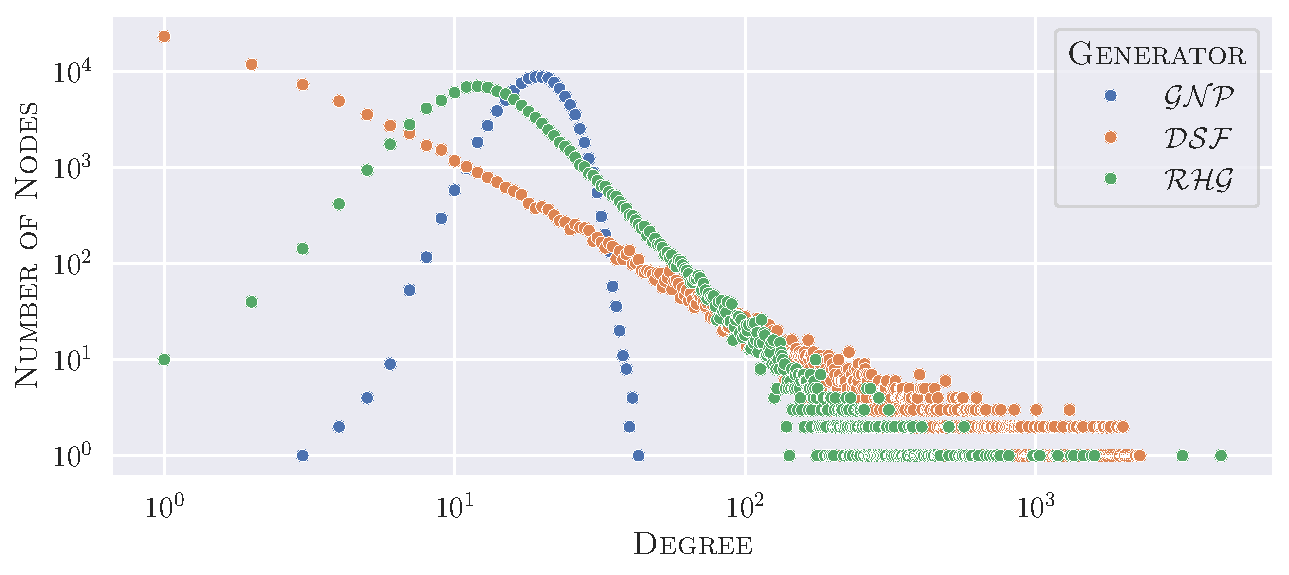
\includegraphics[width=0.85\textwidth]{Figures/Preliminaries/degrees.pdf}
  \caption{Degree distributions for different random graph models with $100 000$ nodes and average degree $20$.}
  \label{fig:degrees}
\end{figure}

\cref{fig:degrees} shows the degree distributions for the three proposed models.
It clearly illustrates that \gnp graphs are not fit to model \qq{scale-free} networks as their degree distribution is a binomial distribution.


\section{Parallel Algorithms}
Parallel algorithms extend the underlying sequential machine model by allowing multiple operations to be done in parallel at the same time.
For that, we can utilize up to $p$ processing units (PUs) that can run computations in parallel.
Although there are multiple models with different restrictions and capabilities, we restrict ourselves to a model where multiple PUs can read data in parallel without interfering so long as this data is not currently being modified.
We however do not allow multiple PUs to change specific values at the same time.\footnote{In the PRAM-Architecture~\cite{PRAM}, this would equate to the CREW-model.}
This eliminates data races and is often the way parallelism is implemented in real machines.

We also only make use of the Fork-Join model~\cite{ForkJoin} in our implementations later in \cref{sec:experiments}.
In the Fork-Join model, we extend the sequential RAM model by two operations: \begin{itemize}
  \item[(Fork)] 
    Split (\emph{fork}) the current task into $N$ new independent parallel subtasks that can run in parallel --- stop the execution of the current task.
  \item[(Join)] 
    Wait for a subset of subtasks to finish their executions and \emph{join} these parallel branches back into a single task.
    This can be accompanied by collecting the data computed by the parallel subtasks.
\end{itemize}
In this model, we can also recursively \emph{fork} subtasks to further subdivide our problem.\footnote{In common implementations of this model, (Fork) only creates $2$ subtasks. Thus to allow for $p$ PUs, we often \emph{fork} $\Th{\log p}$ times (in parallel) to divide the problem into $p$ subtasks.}
For us, in an algorithmic context, the exact method of parallelizing is however not that relevant as it often leads only to constant additional operations since we restrict ourselves to constant number of PUs.

\medskip

For an algorithmic problem $\mcal{A}(n)$, let $\mcal{S}$ denote a sequential algorithm solving $\mcal{A}(n)$ and $\mcal{P}$ denote a parallel algorithm solving $\mcal{A}(n)$ using $p$ PUs.
Let $\rtime_{\mcal{S}}(n)$ and $\rtime_{\mcal{P}}(n)$ denote their respective runtimes.

\begin{definition}[Work]
  The work $W_{\mcal{P}}(n)$ of a parallel algorithm $\mcal{P}$ is the running time $\rtime_{\mcal{P}}(n)$ times the number of PUs $p$ used, \ie \[
    W_{\mcal{P}}(n) \Def p \cdot \rtime_{\mcal{P}}(n).
  \] 
\end{definition}

Thus, $W_{\mcal{P}}(n)$ is the total number of operations of $\mcal{P}$ on inputs of size $n$ (asymptotically).
This gives a direct bound on the work if $\mcal{S}$ is the fastest possible algorithm solving $\mcal{A}(n)$ since simulating the work of $p$ PUs sequentially leads to no more total work.

\begin{observation}\label{obs:work_bounded}
  If $\mcal{S}$ is the fastest sequential algorithm solving $\mcal{A}(n)$, then \[
    W_{\mcal{P}}(n) = \Om{\rtime_{\mcal{S}}(n)}
  \] for every parallel algorithm $\mcal{P}$ solving $\mcal{A}(n)$.
\end{observation}

\noindent We say a parallel algorithm $\mcal{P}$ is work-optimal if $W_{\mcal{P}}(n) = \Th{\rtime_{\mcal{S}}(n)}$.

Another way to analyze parallel algorithms is to formalize the gain we get by using a parallel algorithm $\mcal{P}$ instead of a sequential algorithm $\mcal{S}$.

\begin{definition}[Speedup]
  The speedup $S_{\mcal{S}, \mcal{P}}(n)$ of a parallel algorithm $\mcal{P}$ over a sequential algorithm $\mcal{S}$ is defined as \[
    S_{\mcal{S}, \mcal{P}}(n) \Def \frac{\rtime_{\mcal{S}}(n)}{\rtime_{\mcal{P}}(n)}.
  \]
\end{definition}

Note that in practice the notion of a speedup often only makes sense if either $\mcal{S}$ is the fastest sequential algorithm for $\mcal{A}(n)$ or $\mcal{P}$ is a direct parallelization of $\mcal{S}$, \ie $\mcal{P}$ performs the exact same steps as $\mcal{S}$ with some possibly additional steps (but not less!).
For the rest of the thesis, we assume that at least one of these holds true.
We can extend \cref{obs:work_bounded} to speedups.

\begin{observation}
  For a parallel algorithm $\mcal{P}$ with $p$ PUs and a sequential algorithm $\mcal{S}$, always \[
    S_{\mcal{S}, \mcal{P}}(n) = \Oh{p}.
  \]
\end{observation}


\section{Markov Chains}
\begin{figure}[t]
  \centering
  \begin{tikzpicture}
    \node[vertex] (a) at (0,0) {$1$};
    \node[vertex] (b) at (2,2) {$2$};
    \node[vertex] (c) at (4,0) {$3$};

    \edge{a}{b}{$0.5$}{}{bend left};
    \edge{b}{c}{$1$}{}{bend left};
    \edge{c}{b}{$0.5$}{}{bend left};
    \edge{c}{a}{$0.5$}{}{};
    \path[edge, loop left] (a) to node {$0.5$} (a);
\end{tikzpicture}

  
  \caption{
    A \markov with $3$ states. 
  }
  \label{fig:markov_example}
\end{figure}

Markov chains are a widely studied and adopted model for dynamic random processes~\cite{MCApp1,MCApp2,DBLP:conf/alenex/GkantsidisMMZ03,DBLP:conf/alenex/StantonP11}.
They are \qq{memoryless} since every transition only depends on the current state and input which often makes them a great modeling choice~\cite{MarkovMemoryless}.

\begin{definition}[Stochastic Matrix]
  A matrix $P \in \sR^{n \times n}$ with $n \in \sN$ is called stochastic if $P_{i, j} \in [0, 1]$ for all $i, j \in [n]$ and \[
    \sum_{j = 1}^{n}P_{i, j} = 1 \quad \forall i \in [n].
  \] We sometimes write $P(i, j)$ instead of $P_{i,j}$.
\end{definition}

\noindent A stochastic matrix can model transition probabilities.
Each row $i \in [n]$ then represents the current state $i$ and each column $j \in [j]$ in row $i$ then represents the probability of transitioning from state $i$ to state $j$.
Fixing an arbitrary order for elements of a set, we can model transition probabilities between elements of arbitrary (finite) sets.

\begin{definition}[Markov Chain~\cite{MarkovChainsOrig}]
  A \markov is a tuple $\mathcal{M} = (\states, P)$ where $\states$ is a (finite) set of states and $P \in [0, 1]^{|\states| \times |\states|}$ is a stochastic matrix.
  $P$ defines transition probabilites between states of $\states$, \ie $P_{i, j}$ is the probability to transition from state $i \in \states$ to $j \in \states$.
\end{definition}

\noindent In \cref{fig:markov_example} for example, we have $\states = \set{1, 2, 3}$ and transition probabilities \[
  P = \left(\begin{array}{ccc}
    \frac{1}{2} & \frac{1}{2} & 0 \\
    0 & 0 & 1 \\
    \frac{1}{2} & \frac{1}{2} & 0 
  \end{array}\right).
\]

\noindent While we formalize \markovs here using a finite state set and transition matrix, we can also model transition matrices and consequently \markovs for countable infinite sets of states \states.
Furthermore, we often describe a transition matrix and thus its \markov only with its non-zero transition probabilities without formalizing the complete transition matrix.

\begin{definition}[Distribution]
  A vector $\pi \in [0, 1]^{|\states|}$ is a distribution over states of the \markov if $\norm{\pi} = 1$.
\end{definition}

\noindent A distribution can represent the probabilities in which state the \markov is currently in.
Typically, in the beginning, this is deterministic with $\pi_i = 1$ for some $i$ and $\pi_j = 0$ for every other $j \neq i$.
After one step, we might end up in different states depending on the transition probabilities.
Thus, the distribution is no longer deterministic if we make non-deterministic steps.

\begin{definition}[Random Walk]
  A random walk starts in any distribution over states $\pi^{(0)} \in [0, 1]^{|\states|}$ and applies the transition matrix iteratively, \ie makes a random step based on $P$ \[
    \pi^{(k + 1)} = P \cdot \pi^{(k)} = P^2 \cdot \pi^{(k - 1)} = \cdots = P^{k + 1} \cdot \pi^{(0)}.
  \]
\end{definition}

\begin{definition}[Stationary Distribution]
  A distribution $\pi$ over states is stationary if $\pi = P \cdot \pi$.
\end{definition}

\noindent For example, $\pi = \left(\frac{1}{3}, \frac{1}{3}, \frac{1}{3}\right)$ is a stationary distribution for the \markov in \cref{fig:markov_example}.
It can be shown that for certain \markovs, a stationary distribution $\pi$ always exists and every random walk converges to $\pi$ independent of its initial distribution.

\begin{definition}[Irreducible]
  A \markov is irreducible if the underlying state graph is strongly connected.
\end{definition}

\begin{definition}[Aperiodic]
  A \markov is aperiodic if for every state $i$ the greatest common divisor for the length of all cycles starting in $i$ in the underlying state graph is $1$.
\end{definition}

\noindent We also call a \markov with these two properties \emph{ergodic}.

\begin{observation}\label{obs:loop_implies_aperiodic}
  A irreducible \markov is aperiodic if the underlying state graph has a self-loop.
\end{observation}

\begin{lemma}[\cite{MarkovChainsOrig,MarkovErgodicProof}]
  If a \markov is irreducible and aperiodic, a unique stationary distribution $\pi$ exists and every random walk converges to $\pi = \pi^{(\infty)}$.
\end{lemma}

If the \markov is not irreducible, there are some states we cannot reach from other states, thus there might be more than one stationary distribution if the underlying state graph consists of multiple SCCs.
If the \markov is not aperiodic, then every distribution alternates between different regimes of the \markov and every random walk diverges.
There are some \markovs that do not have both these properties but have a unique stationary distribution to which every random walk converges\footnote{
  For example: consider the \markov in \cref{fig:markov_example} and add a new node $4$ with edge $(4, 1)$ and transition probability $1$.
  Then, the \markov is no longer irreducible but $\pi = \left(\frac{1}{3}, \frac{1}{3}, \frac{1}{3}, 0\right)$ is (still) the unique stationary distribution to which every random walk converges to.
}.

We introduce one other important property that further simplifies the computation of a stationary distribution $\pi$. 

\begin{definition}[Symmetric]
  A \markov is symmetric if $P_{i, j} = P_{j, i}$ for every $i, j \in S$.
\end{definition}

\begin{lemma}[Th. 7.10 from~\cite{DBLP:books/daglib/0012859}]\label{lem:sym_mc_uniform}
  A \markov that is irreducible, aperiodic, and symmetric converges to the uniform distribution over $\states$.
\end{lemma}

\noindent While every \markov satisfying these properties eventually converges to its stationary distribution $\pi$, for different \markovs, it might take longer to get closer to $\pi$ than others.
Thus, we also want to have a measure of how fast a \markov actually converges, \ie how many steps it takes to get arbitrarily close to $\pi$.

\begin{definition}[MixingTime]\label{def:mixing_time}
  For $\epsilon > 0$, the mixing time \mixtime of an ergodic \markov with stationary distribution $\pi$ is defined as \[
    \mixtime = \min\set{\tau \geq 0 \colon \max_{x \in \states}\left[\sum_{y \in \states}|\pi(y) - \sigma_{\tau, x}(y)| \leq \epsilon\right]}
  \] where $\sigma_{\tau, x}$ is the distribution of the \markov after $\tau$ steps starting in distribution $x$.
\end{definition}

\noindent We say a \markov is rapidly mixing if \mixtime is bounded by a polynomial in \[
  \frac{\log|\states|}{\epsilon}.
\]

\begin{examplesketch}[\mixtime of \cref{fig:markov_example}]
  For the \markov in \cref{fig:markov_example}, we have \[
    \ceil{\lb{\frac{1}{\epsilon}} + \lb{\frac{2}{3}}} \leq \mixtime \leq \ceil{\lb{\frac{1}{\epsilon}} + 1}
  \]
\end{examplesketch}
\begin{proof}
  Notice that $\sigma_{\tau, x} = P^{\tau}x$.
  We can prove by induction that we have \[
    P^{\tau} = \frac{1}{2^k}\begin{cases}
      \left(\begin{array}{ccc}
        \Delta_k + 1 & \Delta_k + 1 & \Delta_k \\
        \Delta_k & \Delta_k & \Delta_k + 2 \\
        \Delta_k + 1 & \Delta_k + 1 & \Delta_k
    \end{array}\right) & \text{if $k$ is odd} \\
    \left(\begin{array}{ccc}
        \Delta_k & \Delta_k & \Delta_k + 1 \\
        \Delta_k + 1 & \Delta_k + 1 & \Delta_k - 1 \\
        \Delta_k & \Delta_k & \Delta_k + 1 
    \end{array}\right) & \text{if $k$ is even}
    \end{cases}.
  \] for $\Delta_k = \frac{2^k - 1 - \left(k \mod 2\right)}{3}$.
  Then, simply bound $|\pi - P^{\tau}x|$ from below and above to get the stated bounds.
\end{proof}
